%!TEX TS-program = xelatex
%!TEX encoding = UTF-8 Unicode
\documentclass[landscape,a1paper,fontscale=0.42]{baposter}

\usepackage[vlined]{algorithm2e}
\usepackage{times}
\usepackage{calc}
\usepackage{url}
\usepackage{graphicx}
\usepackage{amsmath}
\usepackage{amssymb}
\usepackage{relsize}
\usepackage{multirow}
\usepackage{booktabs}

\usepackage{graphicx}
\usepackage{multicol}
\usepackage[T1]{fontenc}
\usepackage{ae}
\usepackage{enumitem}

\usepackage{colortbl}
\usepackage{xcolor}
%\usepackage{gensymb} % for \degree
\graphicspath{{images/}}

\setlist[itemize]{leftmargin=*,nosep}
    \setlength{\columnsep}{0.7em}
    \setlength{\columnseprule}{0mm}

\setlist[enumerate]{leftmargin=2.5em,nosep}
    \setlength{\columnsep}{1.0em}
    \setlength{\columnseprule}{0mm}


\definecolor{darkcyan}{HTML}{bfd8d9}
\definecolor{ctitle}{HTML}{0c3436}

% %%%%%%%%%%%%%%%%%%%%%%%%%%%%%%%%%%%%%%%%%%%%%%%%%%%%%%%%%%%%%%%%%%%%%%%%%%%%%%%%
% % Save space in lists. Use this after the opening of the list
% %%%%%%%%%%%%%%%%%%%%%%%%%%%%%%%%%%%%%%%%%%%%%%%%%%%%%%%%%%%%%%%%%%%%%%%%%%%%%%%%
% \newcommand{\compresslist}{%
% \setlength{\itemsep}{0pt}%
% \setlength{\itemsep}{0pt}%
% \setlength{\parskip}{0pt}%
% \setlength{\parsep}{0pt}%
% }
\renewcommand{\rmdefault}{ptm} % Arial
\renewcommand{\sfdefault}{ptm} % Arial

\newcommand{\Sys}{\textsc{Opera}\xspace}
\newcommand{\Cache}{\textsc{HomCache}\xspace}

%%%%%%%%%%%%%%%%%%%%%%%%%%%%%%%%%%%%%%%%%%%%%%%%%%%%%%%%%%%%%%%%%%%%%%%%%%%%%
%% Begin of Document
%%%%%%%%%%%%%%%%%%%%%%%%%%%%%%%%%%%%%%%%%%%%%%%%%%%%%%%%%%%%%%%%%%%%%%%%%%%%%
\begin{document}
%%%%%%%%%%%%%%%%%%%%%%%%%%%%%%%%%%%%%%%%%%%%%%%%%%%%%%%%%%%%%%%%%%%%%%%%%%%%%
%% Here starts the poster
%%---------------------------------------------------------------------------
%% Format it to your taste with the options
%%%%%%%%%%%%%%%%%%%%%%%%%%%%%%%%%%%%%%%%%%%%%%%%%%%%%%%%%%%%%%%%%%%%%%%%%%%%%
\begin{poster}{
    % Show grid to help with alignment
    grid=false,
    columns=5,
    % Column spacing
    colspacing=0.7em,
    % Color style
    headerColorOne=darkcyan,
    borderColor=darkcyan,
    % Format of textbox
    textborder=faded,
    % Format of text header
    headerborder=open,
    headershape=roundedright,
    headershade=plain,
    background=none,
    bgColorOne=cyan!10!white,
    headerheight=0.13\textheight
}
% Eye Catcher
{
    \makebox[0.01\textwidth]{}
    
\includegraphics[width=0.05\linewidth]{logo/HKU_logo}
    \makebox[0.03\textwidth]{}
    \raisebox{0.08\height}{
\includegraphics[width=0.05\linewidth]{logo/Huawei_logo}}
}
% Title
{
    \huge\bf \Sys{}: Achieving Secure and High-performance OLAP with Parallelized Homomorphic Comparisons
}
% Authors
{
    \vspace{0.3em}
        Qi Hu$^{1\dagger}$ \enspace
        Wei Chen$^{1\dagger}$ \enspace
        Tianxiang Shen$^{21*}$ \enspace
        Xin Yao$^{2}$ \enspace
        Nicholas Zhang$^{2}$ \enspace
        Heming Cui$^{1*}$ \enspace
        Siu-Ming Yiu$^{1}$ \\
    {$^{1}$The University of Hong Kong \enspace$^{2}$Huawei Technologies Co., Ltd.} \\
    {\normalsize $^\dagger$Equal contribution. $^*$Co-corresponding authors.}
}
% University logo
{
    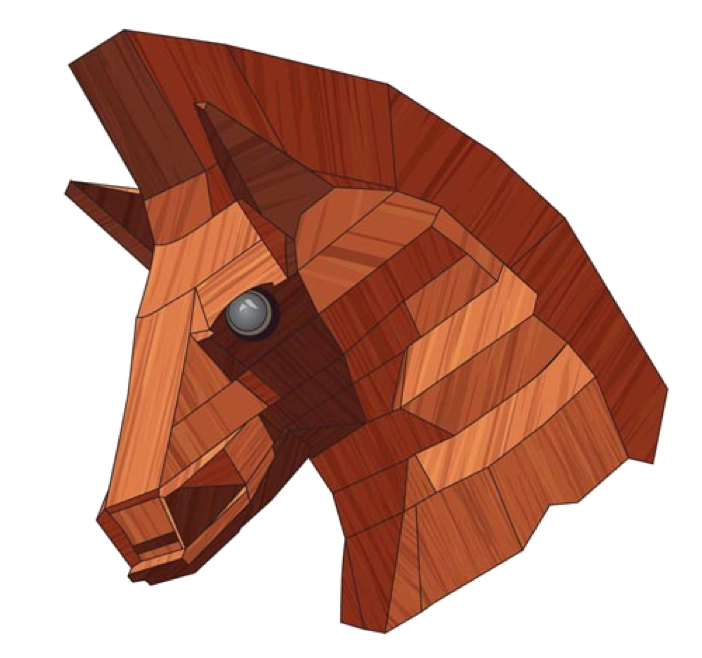
\includegraphics[width=0.08\linewidth]{logo/trojan.png}
    \makebox[0.01\textwidth]{}
}

%%%%%%%%%%%%%%%%%%%%%%%%%%%%%%%%%%%%%%%%%%%%%%%%%%%%%%%%%%%%%%%%%%%%%%%%%%%%%%
%%% Now define the boxes that make up the poster
%%%---------------------------------------------------------------------------
%%% Each box has a name and can be placed absolutely or relatively.
%%% The only inconvenience is that you can only specify a relative position 
%%% towards an already declared box. So if you have a box attached to the 
%%% bottom, one to the top and a third one which should be inbetween, you 
%%% have to specify the top and bottom boxes before you specify the middle 
%%% box.
%%%%%%%%%%%%%%%%%%%%%%%%%%%%%%%%%%%%%%%%%%%%%%%%%%%%%%%%%%%%%%%%%%%%%%%%%%%%%%

%%%%%%%%%%%%%%%%%%%%%%%%%%%%%%%%%%%%%%%%%%%%%%%%%%%%%%%%%%%%%%%%%%%%%%%%%%%%%%
\headerbox{\bf\color{blue} Problem Definition and Contribution}{name=contribution,column=0,row=0,span=2}{
    
}

\headerbox{\bf\color{blue} Problem Formulation}{name=formulation,column=0,below=contribution,span=2}{
    
}

\headerbox{\bf\color{blue} Method}{name=abstract,column=0,below=formulation,span=2}{
    
}
%
\headerbox{\bf\color{blue} Experiments \& Results}{name=results,column=2,row=0,span=3}{
    
}
\end{poster}
\end{document}